\section{Job management service}\label{section:jms}

Job management service (JMS) responsibilities are:

\begin{itemize}
\item Keeping track of all registered components
\item Accepting submitted jobs
\item Distributing jobs among all components involved
\end{itemize}

\subsection{Requirements and Dependencies}

Job management service requires the following tools for it's proper function:

\begin{itemize}
    \item Kafka 2.4.0
    \item .Net Core 3.1.100
\end{itemize}

It communicates with the following service:
\begin{itemize}
    \item Storage service (see Section \ref{section:storage})
\end{itemize}

\subsection{Code}

JMS is web application running on ASP .NET Core 3.1 which implement standard Model-View-Controller principle. The solution follows domain-drive-principle\footnote{\url{https://docs.microsoft.com/en-us/dotnet/architecture/microservices/microservice-ddd-cqrs-patterns/ddd-oriented-microservice}} which requires  the code base into the following projects: 
\begin{itemize}
    \item \texttt{Api} - entry point of the application, contains configuration \texttt{appsettings.json} and controllers handling http requests
    \item \texttt{Domain} - business logic, platform independent
    \item \texttt{Infrastructure} - platform dependent implementation
    \item \texttt{Tests} - unit tests and integration tests
\end{itemize}

Application uses dependency injection that is configured in the project \texttt{Api} in the file  \texttt{JobManagementServiceBuilder.cs}.

JMS main domain is to manage jobs invoked via HTTP interface. Each job is performed by component. Since the components are not known in advance, each component needs to registered itself via Kafka interface. JMS is stateless, all the data is stored in storage service. The major components of JMS can bee seen in the Figure \ref{figure:class-jms}.
 
\paragraph{Major Classes}

\begin{itemize}
    \item \texttt{JobController} - The controller responsible for processing job related requests
    \item \texttt{SubscribedComponentManager} - Contains the vital logic of JMS implemented by the method \texttt{StartJobAsync}. Also used for registering components
    \item \texttt{RegistrationRequestListener} - Continuously listens to the topic\\ \texttt{job\_management.registration.request}. It is used by all other components to register themselves (for more details refer to Section \ref{subsubsection:jms_kafkainterface}). 
    \item \texttt{RegistrationRequestProcessor} - Parses registration requests and stores it in the database
    \item \texttt{StorageService} - Used as a proxy to storage service (see Section \ref{section:storage})
\end{itemize}

\begin{figure}
    \centering
    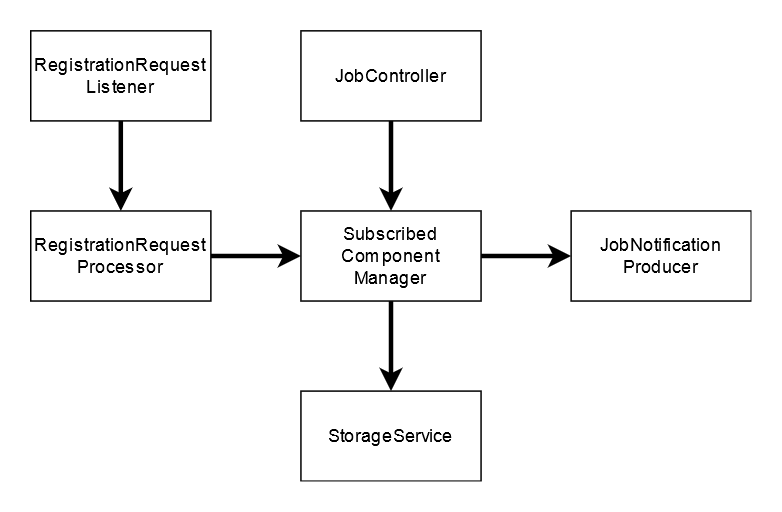
\includegraphics[width=0.9\textwidth]{diagrams/class-jms.png}
    \caption{The diagram shows relationships among major classes of JMS}
    \label{figure:class-jms}
\end{figure}

\subsection{Configuration}

The configuration of JMS is stored in the project \texttt{Api} in the file \texttt{appsettings.json}. It does not require any user's input. The configuration is distributed via a dependency injection container. Each option of the configuration needs to be bound to the file. This binding is in the project \texttt{Api} in the file  \texttt{JobManagementServiceBuilder.cs}.

The most notable configuration objects:

\begin{itemize}
    \item \texttt{KafkaOptions} - contains URI of Kafka. In case of starting JMS differently then advised, this element would need to be changed. (for \texttt{localhost} for example).
    \item \texttt{JobStorageOptions}, \texttt{StorageServiceHealtcheckOptions}, \texttt{Component\-StorageOptions} - these objects contain endpoint routes for the storage service. 
    \item \texttt{StorageChannelNames} - names of Kafka topics used to propagate posts and analyses to the storage.
\end{itemize}

\subsection{Build + Run}

Navigate to the source code, specifically to the \texttt{job-management/Api} type in the following commands:

\begin{itemize}
    \item \texttt{dotnet restore} - downloads all third party libraries
    \item \texttt{dotnet build} - build the projects
    \item \texttt{dotnet run} - run the projects
\end{itemize}

\subsection{Communication}\label{subsection:jms_communication}
\begin{figure}[H]
    \centering
    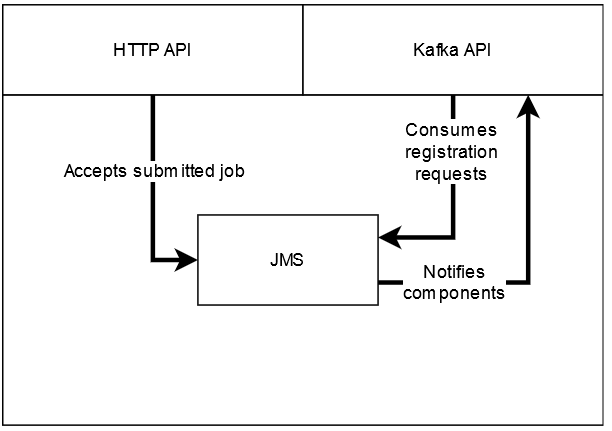
\includegraphics[width=0.8\textwidth]{diagrams/api-jms.png}
    \caption{HTTP interface is used to start or stop jobs. Kafka interface is used to listen to registration requests}
    \label{fig:apiJms}
\end{figure}
JMS uses Kafka and HTTP for communication depicted in Figure \ref{fig:apiJms}.



\subsubsection{Kafka Interface}\label{subsubsection:jms_kafkainterface}

Kafka is used to listen for registration request of the JSON format on the topic \texttt{job\_management.registration.request} from all components. 

The registration request (see Appendix \ref{subsection:registrationrequest}) of a component must contain the following fields:

\begin{itemize}
    \item \texttt{componentType} - either \texttt{DATA\_ACQUIER} or \texttt{DATA\_ANALYSER} depending on the type of the component.
    \item \texttt{componentId} - unique id of the component
    \item \texttt{inputChannelName} - name of the channel unique to the component. The component will use it for ingesting the data (in case of acquirer, this field is \texttt{null}.
    \item \texttt{updateChannelName} - name of the channel that the component uses for accepting job notifications.
    \item \texttt{attributes} - an object contains any other attributes
\end{itemize}

\subsubsection{HTTP Interface}\label{subsubsection:jms_httpinterface}

JMS offers two endpoints accepting POST requests:

\begin{itemize}
    \item \texttt{/api/job/submit} - starts jobs and notifies all components
    \item \texttt{/api/job/stop/<jobId>} - stops the jobs on all the components. Has no payload.
\end{itemize}

Submitting a job requires a body with the JSON payload with the following fields:

\begin{itemize}
    \item \texttt{selectedDataAnalysers} - component ids of all selected analysers. If any analyser has not been registered yet, the request fails.
    \item \texttt{selectedDataAcquirers} - same but with acquirers.
    \item \texttt{topicQuery} - topic of interest.
    \item \texttt{jobName} - human readable name.
    \item \texttt{attributes} - custom attributes of selected components. If user wants the component to receive some attributes, the JSON object with the attributes must be wrapped with an element with the component id. 
\end{itemize}

\subsubsection{Outgoing Communication}

JMS sends job notifications to the components via Kafka. Each registered component has a topic on which it listens to job configuration. When the job (see Section \ref{subsubsection:jms_httpinterface}) is submitted, all components involved are sent a job notification (see Appendix \ref{subsection:notification}). The components that re-register themselves receive all active job configurations. This prevents allow crashing components to continue on unfinished jobs.
